\section{A Picard Iteration for the \MA equation}

For quasilinear PDEs such as $\nabla \cdot (A(u) \nabla u ) = f$ it is common to determine the solution via a fixed point iteration. \todo{cite}The key aspect lies in a decoupling of the coefficient matrix $A(u)$ and $\nabla u$. Hence, one solves the equations
\[
	\nabla \cdot (A(u^{i} )\nabla u^{i+1}) = f  \text{ and } \nabla \cdot (A(u^{i+1}) \nabla u^{i}) = f, \text{ respectively}
\] 
iteratively.

In this spirit we want to decouple the derivates in the \MA equation. Recall, the \MA equation states
\begin{align}
 \mydet{D^2 u} &= f \nonumber \\
 	\Leftrightarrow \qquad  \dxx{x_1} u \dxx{x_2} u -\dxy {x_1}{x_2} u \dxy{x_2}{x_1} u  &= f. \label{eq:mongeAmpere detForm}
\end{align}
To shorten and facilitate terms we will denote $x \in \Omega \subset {\R^2} $ by $(x,y)^t$ and the partial derivates with subscripts as for example $\dxx{x_1} u = u_{xx}$.

At first, we multiply \eqref{eq:mongeAmpere detForm} by $2$ and expand the left-hand side
\begin{align}
% 	2\dyy u {x} \dyy u {y}-2\dyx u {x}{y} \dyx u{y}{x}  &= 2 f \\
 	\dyy u {x} \dyy u {y}+\dyy u {x} \dyy u {y} -\dyx u {x}{y} \dyx u{y}{x} -\dyx u {x}{y} \dyx u{y}{x} &=2 f. 
\end{align}

Decoupling into the two functions $v = u ,w = u$ and reordering terms we have
\begin{align}
	w_{yy} v_{xx}- w_{xy} v_{yx} - w_{yx} v_{xy} +w_{xx} v_{yy} = 2f \label{eq:decoupled PDE start}
\end{align}
Rewriting this by matrix frobenius product yields to
\begin{align}
 \begin{pmatrix} w_{yy} & -w_{xy}  \\ -w_{yx} & w_{xx} \end{pmatrix}: \begin{pmatrix} v_{xx} & v_{yx}  \\  v_{xy} & v_{yy} \end{pmatrix} = 2f.
\end{align}
We see that the left matrix is the cofactor matrix of the hessian (Definition \ref{def: cof matrix}) and the right one the hessian itself and find
\begin{align}
		\mycof {D^2 w }:D^2 v  = 2f  \label{eq:short formula}
\end{align}
Note, that this derivation of decoupling of $v,w$ is chosen for it is a very intuitive approach. Alternatively \eqref{eq:short formula} can quickly be derived from the identity $\mycof {D^2 u }:D^2 u  = d \mydet{D^2 u}$ of Lemma \ref{la: rel det cofactor}

Substituting the identity of Lemma \ref{la: An application of the divergernce product rule} and multiplying with -1 we find
\begin{align}
	- \nabla \cdot \left( \mycof{ D^2 w} \nabla v \right)  = -2f.  \label{eq:decoupled PDE}
\end{align}
For a fixed $w$ the left-hand side now is quasilinear in $v$ opposed to the nonlinearity in $u$ in the original PDE. From its derivation it is clear that for smooth functions $w=u, v=u$ \eqref{eq:decoupled PDE} is equivalent to the classical formulation of the \MA equation. Furthermore due to the symmetry of \eqref{eq:decoupled PDE start} in $v$ and $w$, analogously the equation 
\begin{align}
	- \nabla \cdot \left( \mycof{ D^2 v} \nabla w \right)  = -2f.  \label{eq:decoupled PDE two}
\end{align}
can be deduced.

Thus, it is natural to examine the fixed point iteration
\begin{align}
	\begin{split}
	- \nabla \cdot \left( \mycof{ D^2 u^i} \nabla u^{i+1} \right)  &= -2f  \text{ in } \Omega \\
		u^{i+1} &= g \textnormal{ on } \partial \Omega
	\label{eq:fixed point iteration}
	\end{split}
\end{align}
for its applicability for numerical schemes approximating a \MA solution.

\section{SIPG formulation of the Iteration}\label{sec: SIPG MA}
Since in every iteration \eqref{eq:fixed point iteration} states a generalised poisson equation we can apply the derived  SIPG method of section \ref{sec: SIPG} directly: Given $u^i_h$ find $u^{i+1}_h \in \mathcal P^k_h$ satisfying
\begin{align}
 &\int_{\Omega} \nabla v_h \cdot \cof(D_h^2 u_h^{i}) \nabla u_h^{i+1}  \nonumber\\
 & -\sum\limits_{e \in \bigEps^i}\int_{e} \jump {v_h \average { \cof(D_h^2 u^{i}) \nabla u_h^{i+1}} }
 - \sum\limits_{e \in \bigEps^i}\int_{e} \jump {u \average{ \cof(D^2 u_h^{i}) \nabla v_h} } \nonumber\\  
 & - \sum\limits_{e \in \bigEps^b}\int_{e} v_h \cof(D^2 u_h^{i}) \nabla u_h^{i+1}\cdot n 
    - \sum\limits_{e \in \bigEps^b}\int_{e} u_h^{i+1}\cof(D^2 u_h^{i}) \nabla v_h \cdot n
    +\sum\limits_{e \in \bigEps} \int_e \frac \sigma {|e|} \jump {v_h}  \jump {u_h^{i+1}}\nonumber\\
    =& - 2 \int_{\Omega}v_h f
    	 				-\sum\limits_{e \in \bigEps^b}\int_{e} u_h^0 \cof(D^2 u_h^{i}) \nabla v_h \cdot n 
    	 				+\sum\limits_{e \in \bigEps^b} \int_e \frac \sigma {|e|} v_h u_h^0    \qquad \forall v_h \in  \mathcal P^k_h.
    	\label{eq: sipg iteration}
\end{align}

Brenner et. alter emphasised that a convergent scheme needs to retain the consistency between the discretisation of the linearisation and the linearisation of the discretisation. Since the linearisation of the \MA operator is $\nabla \cdot \left( \cofHess u \nabla v \right)$ (cf. Theorem \ref{thm: linearisation}) the stiffness bilinear form of the SIPG method is the linearisation of the \MA equation at $u_i$. Therefore it is consistent if $u_i$ equals the exact solution. 
%
%\section{Wellposedness of the method}
%
%The stability of the linearisation, i.e. an iteration step follows from the fact that the SIPG method is stable with the General Poisson problem. As before we denote the polynomial degree of the ansatz space $V_h=\mathcal P_h^k$ by $k$. We denote further the function space $H^2(\Omega; \triang) \cap H^1(\Omega)$ by $V$. 
%
%Let $L_u:V \rightarrow V'$ for $u \in V$ be the defined by the left hand side of an iteration step, namely
%\begin{align}
%	\bilin {L_u w} v =   &\int_{\Omega} \nabla v \cdot \cof(D_h^2 u) \nabla w \nonumber\\
%	& -\sum\limits_{e \in \edges}\int_{e} \jump {v \average { \cof(D_h^2 u) \nabla w} }
%	- \sum\limits_{e \in \edges}\int_{e} \jump {u \average{ \cof(D^2 u) \nabla v} } \nonumber\\  
%	&+\sum\limits_{e \in \edges} \int_e \frac \sigma {|e|} \jump {v}  \jump {w}
%\end{align}
%Furthermore let $L_{u,h}:V_h \rightarrow V_h'$ be the restriction from $L_u$ to $V_h$. 
%Since for convex $u$ the cofactor matrix is always positive definite we showed in Theorem \ref{thm: SIPG stability} that $L_{u,h}$ is invertible. We denote its inverse by $L_{u,h}^{-1}$.
%
%The following lemma follows directly from the definition of $L_u$
%\begin{lemma}\label{la: addition L}
%	For $u,v \in V$ holds
%	\[
%		L_{u+v}w = L_{u}w + L_{v}w - Jw
%	\]
%	where $J \in V'$ is given by
%\[
%	\bilin {Jw} v = \sum\limits_{e \in \edges} \int_e \frac \sigma {|e|} \jump {v}  \jump {w} \qquad \forall w \in V
%\] 
%\end{lemma}
%
%Additionally we introduce the functional $R_u \in V'$ for the right-hand side of \eqref{eq: sipg iteration} defined by
%\[
%	\bilin {R_u} v = - 2 \int_{\Omega}v f
%	-\sum\limits_{e \in \edgesb}\int_{e} g \cof(D^2 u) \nabla v \cdot n 
%	+\sum\limits_{e \in \edgesb} \int_e \frac \sigma {|e|} v g
%\]
%
%Our desired Picard iteration fixed point $w_h \in V_h$ is then described by the equation
%\begin{align}
%	\bilin {L_{w_h, h} w_h} v =  \bilin {R_{w_h}} v   \qquad \forall v \in V \label{eq: fixed point functional}
%\end{align}
%or as the fixed point in $V_h$ of the function $F:V \rightarrow V'$ defined by
%\begin{align}
%\bilin {Fu} v =  \bilin {L_u u - R_u} v   \qquad \forall v \in V. \label{eq: root functional}
%% F = L_{w,h}^{-1} R_w
%\end{align}
%
%The goal is to prove \eqref{eq: fixed point functional} has a solution in $V_h$. To this end, we consider for the rest of the analysis a convex and polyhedral domain $\Omega\in \R^2$, a positive $f \in C^{k+1}$ and $g\in C^{k+3}(\partial \Omega)$. By the results of \cite{CNS1984} the \MA problem then has a convex solution $u$. Note, that $u$ denotes from now on a fixed function.
%
%Consider the operator $\mathcal M: V \rightarrow V_h$
%\begin{align}
%	\mathcal M = L_{u,h}^{-1}(L_{u} - F)
%\end{align}
%and let $\mathcal M_h:V_h \rightarrow V_h$ be its restriction to $V_h$. Clearly, $\mathcal M_h$ reduces to 
%\begin{align}
%\mathcal M = id_h - L_{u,h}^{-1}F
%\end{align}
%Since $L_{u,h}$ is a isomorphism the existence of a fixed point of $\mathcal M_h$ implies the existence of a root to \eqref{eq: root functional} and hence a fixed point to our Picard Iteration restriced to $V_h$.
%
%By Lemma \ref{la: addition L} it holds for any $w \in V$ that $L_{u}w = L_{w}w + L_{u-w}w -Jw$. Thus,we have using the definition of $F$ \eqref{eq: root functional}
%\begin{align*}
%	\mathcal M w &= L_{u,h}^{-1}(L_u w - Fw) \\
%				 &= L_{u,h}^{-1}(L_uw - L_w w + R_w)
% \end{align*}
%and hence
%\begin{align*}
%	\HOneDnorm{\mathcal M w_1 - \mathcal M w_2} =& \HOneDnorm{L_{u,h}^{-1}(L_{u}(w_1-w_2)-L_{w_1}w_1+L_{w_2}w_2+ R_{w_1} - R_{w_2})}. \\
%\end{align*}
%Applying theorem \ref{thm: SIPG stability} yields
%\begin{align}
%	\HOneDnorm{\mathcal M w_1 - \mathcal M w_2}	\leq C \HMinusOneDnorm{L_{u}(w_1-w_2)-L_{w_1}w_1+L_{w_2}w_2+ R_{w_1} - R_{w_2} } \label{eq: estimate M}
%\end{align}
%Let us consider the terms separately:
%We have again by theorem \ref{thm: SIPG stability}
%\begin{align}
%\HMinusOneDnorm{L_{u}(w_1-w_2)} \leq C \HOneDnorm{w_1 - w_2}.
%\end{align}	
%It holds 
%\begin{align}
%	\bilin{L_{w_1}w_1-L_{w_2}w_2} v =& \int_{\Omega} \left( \nabla w_1 \cofHess{w_1} \nabla v- \nabla w_2 \cofHess{w_2} \nabla v \right) \nonumber\\
%	& -\sum\limits_{e \in \edges}\int_{e} \left( \jump {v \average { \cof(D_h^2 w_1) \nabla w_1} } 
%					- \jump {v \average { \cof(D_h^2 w_2) \nabla w_2} }\right) \nonumber \\
%	&- \sum\limits_{e \in \edges}\int_{e} \left(\jump {w_1 \average{ \cof(D^2 w_1) \nabla v} } 
%					- \jump {w_2 \average{ \cof(D^2 w_2) \nabla v} }\right)\nonumber\\  
%	&+\sum\limits_{e \in \edges} \int_e \frac \sigma {|e|} \left( \jump {v}  \jump {w_1}-\jump {v}  \jump {w_2} \right).
% \end{align}
%Adding and substracting terms we can rewrite this to
%\begin{align}
%%\bilin{L_{w_1}w_1-L_{w_2}w_2} v =
%& \int_{\Omega} \left( \nabla (w_1-w_2) \cofHess{w_1} \nabla v- \nabla w_2 \cofHess{w_1 - w_2} \nabla v \right) \nonumber\\
%& -\sum\limits_{e \in \edges}\int_{e} \left( \jump {v \average { \cof(D_h^2 w_1) \nabla (w_1-w_2)} } 
%- \jump {v \average { \cof(D_h^2 (w_1-w_2)) \nabla w_2} }\right) \nonumber \\
%&- \sum\limits_{e \in \edges}\int_{e} \left(\jump {(w_1-w_2) \average{ \cof(D^2 w_1) \nabla v} } 
%- \jump {w_2 \average{ \cof(D^2 (w_1-w_2)) \nabla v} }\right)\nonumber\\  
%&+\sum\limits_{e \in \edges} \int_e \frac \sigma {|e|} \jump {v}  \jump {w_1-w_2}.
%\end{align}
%Therefore it follows with the Cauchy-Schwarz inequality that
%\begin{align}
%\bilin{L_{w_1}w_1-L_{w_2}w_2} v \leq &  \LTwonorm{w_1-w_2} \LTwonorm{\cofHess{w_1}} \LTwonorm{\nabla v} \nonumber\\
%			&+ \LTwonorm{w_2} \LTwonorm{\cofHess{(w_1-w_2)}} \LTwonorm{\nabla{v}} \nonumber \\
%		&+ \sum_{e \in \edges} 
%			\norm{v}_{L^\infty(\Omega)}( %\left(
%				\LTwonormE{ \average{ \cof(D_h^2 (w_1))}} \LTwonormE{ \average{\nabla (w_1-w_2)}} \nonumber\\
%			  &\phantom++\LTwonormE{ \average{ \cof(D_h^2 (w_1-w_2))}} \LTwonormE{ \average{\nabla (w_2)}} 
%			) \nonumber \\%\right)
%		&+ \sum_{e \in \edges} 
%			( %\left(
%				\LTwonormE{ \average{(w_1-w_2)}} \LTwonormE{ \average{ \cof(D_h^2 (w_1))}} \nonumber\\
%				&\phantom++\LTwonormE{ \average{(w_2)}} \LTwonormE{ \average{ \cof(D_h^2 (w_1-w_2))}} 
%		) \norm{\nabla v}_{L^\infty(\Omega)}%\right)
%\end{align}
%Considering the definition of the cofactor matrix it is easy to deduce that $\norm{\cofHess{v}}_* =\norm{D^2_h{v}}_*$ holds.
%Using this fact and Lemma \ref{la: trace estimate} we find
%\begin{align}
%\bilin{L_{w_1}w_1-L_{w_2}w_2} v \leq & %(1+|\ln( h) |^{\frac 1 2 } 
%\LTwonorm{w_1-w_2} \LTwonorm{\hess{w_1}} \LTwonorm{\hess{v}} \nonumber\\
%&+ \LTwonorm{w_2} \LTwonorm{\hess{(w_1-w_2)}} \LTwonorm{\hess{v}} \nonumber \\
%	&+ \sum_{e \in \edges} (
%		\LTwonormE{ \average{ \hess{w_1 }}} \LTwonormE{ \average{\nabla (w_1-w_2)}} \nonumber\\
%		&\phantom+ +\LTwonormE{ \average{ \hess{w_1-w_2}}} \LTwonormE{ \average{\nabla (w_2)}}  \nonumber \\%\right)
%		&\phantom+ +\LTwonormE{ \average{(w_1-w_2)}} \LTwonormE{ \average{ \hess{w_1}}} \nonumber\\
%		&\phantom+ +\LTwonormE{ \average{(w_2)}} \LTwonormE{ \average{ D_h^2 (w_1-w_2)}} 
%	)
%\end{align}


\section{Challenges for a \MA DG method}
Reviewing existing DG methods for the \MA we learned some ?(subjects, matter, points) we have to pay attention to  while examining the fixed point iteration. The next subsections treat the most challenging points.

\subsection{Convexfication} \label{subsec: convexification}
 The \MA equation in general does not define a unique solution. For most applications the unique convex solution is required. The question is there a appropriate method to oblige a numerical method to select only convex solutions.
The most intuitive way is to convexify the solution after every step. Thereby, on one hand we make sure the right solution is approximated and on another hand we smooth the Generalised Poisson solution. This could also improve the quality of second derivatives of our interim solution. % aiming for a better approximation of the second derivatives.
Unfortunately convexification is not simple. For our approach we choose a Bernstein basis for the ansatz space at first.
\begin{definition}[Bernstein-B\'ezier form]\label{def: BernsteinBezierForm}
	Any univariate polynomial of degree $k$ on a triangle $T$ can be represented in \emph{Bernstein-B\'ezier form} as
\begin{align}
	p(x) = \sum_{i+j+k = d}  c_{ijk} B^d_{ijk}(x),\label{eq: BernsteinBezierForm}
\end{align}
where
\[
	B^d_{ijk}(x) = \frac {d!}{i!j!k!} \beta_1^i \beta_2^j \beta_3^k
\]
are the \emph{Bernstein polynomials} of degree $k$ and $\beta = (\beta_1, \beta_2, \beta_3)$ are the barycentric coordinates of $x$ relative to the triangle $T$.
The points $c_{ijk}$ are called \emph{control points} and the polygon defined by the control points \emph{B\'ezier control polygon}.
\end{definition}

The benefit of the Bernstein-B\'ezier form is that there can be formed conditions ensuring the convexity of the polynomial on a triangle. Namely there is a connection between the convexity of the control polygon and the convexity of the polynomial.
\begin{theorem}[ {\cite[Theorem 4.6]{Dahmen1991}}]
	The convexity of the control polygon implies the convexity of the represented polynomial.
\end{theorem}
Note, that this result holds only for a single triangle and not for the convexity of the whole patch. Nevertheless, piecewise convexity is very important for the condition of the Generalised Poisson problem such that it is worth a try to convexify the union of all control polygons.
Due to their importance in computer graphics, there are a lot of convex hull algorithm available. Hence it suggests itself to apply a convex hull algorithm on given Bernstein-B\'ezier coefficients to enforce convexity. However, this approach is designated to go amiss for a convex hull algorithm only operate on a set of point and does not necessarily produce the same connectivity the control polygon implies. An example for that is given in figure \ref{fig: diff connectivity}:
\begin{figure}[h]
\begin{subfigure}[b]{.5\textwidth}
	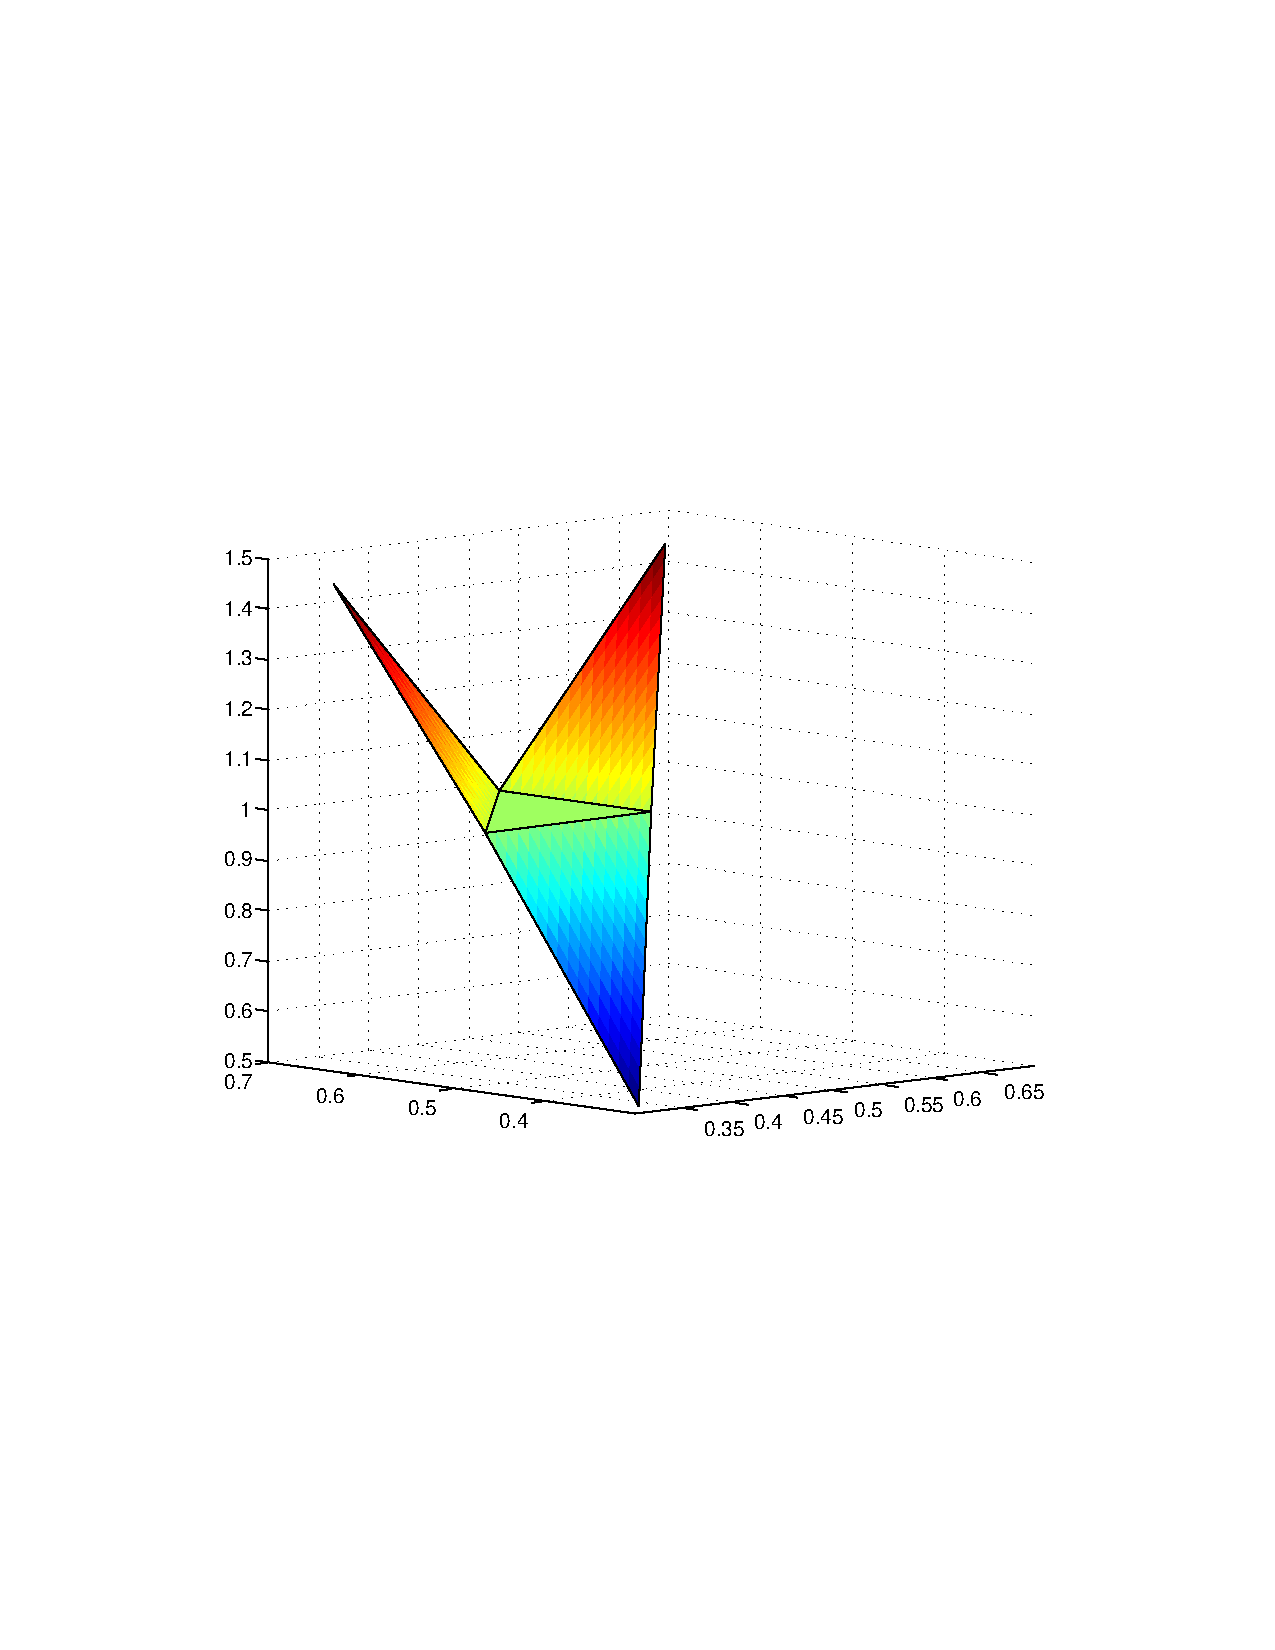
\includegraphics[trim=3cm 8cm 3cm 8cm, width=1.\textwidth]{control_polygon2.pdf}
	\caption{control polygon}
\end{subfigure}
\begin{subfigure}[b]{.5\textwidth}
	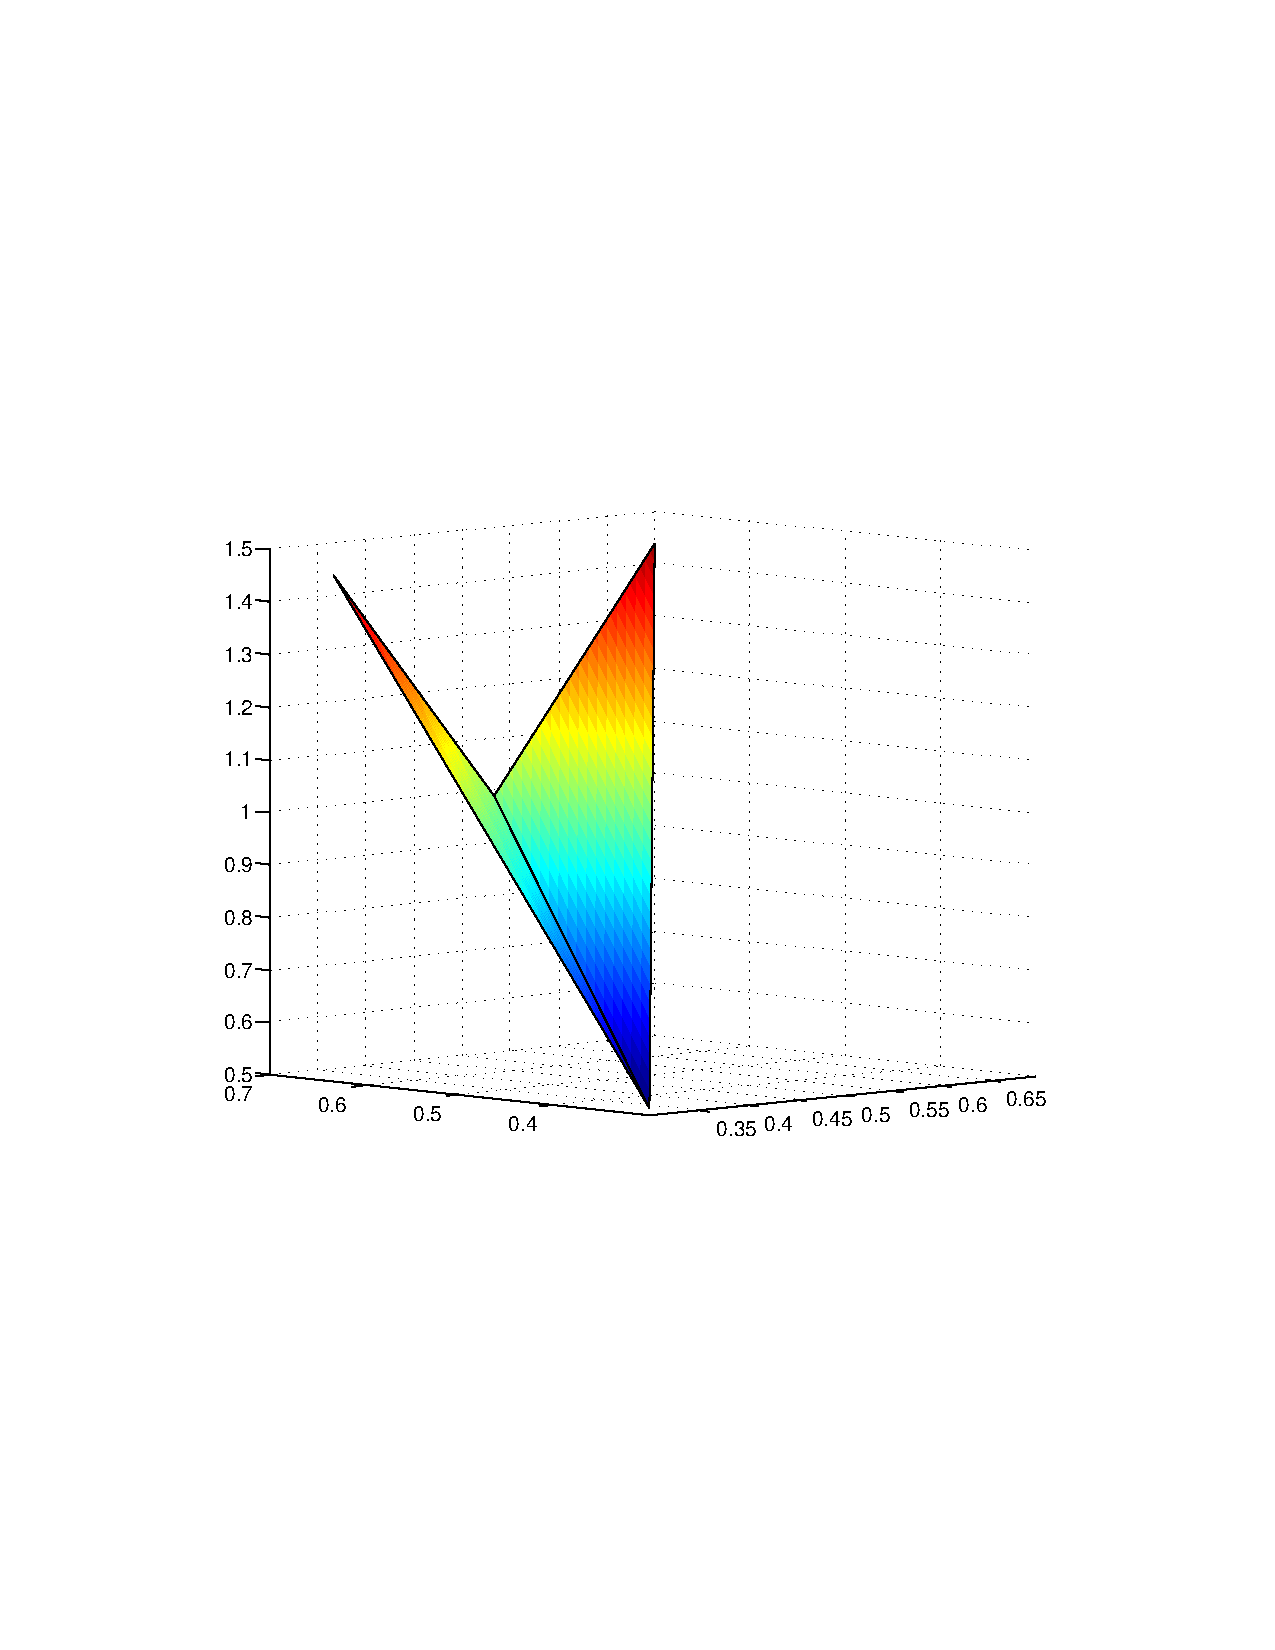
\includegraphics[trim=3cm 8cm 3cm 8cm, width=1.\textwidth]{convex_hull2.pdf}
	\caption{lower convex hull}
\end{subfigure}
\caption{The control polygon and lower convex hull of a given set of control points}
\label{fig: diff connectivity}
\end{figure}
While the the control polygon is obviously not convex, the surface of the lower convex hull of the control points is convex because it connects the inner control points differently.

\todo{altere idee nur fur c0 splines}
In the eighties mathematicians pursuit an approach based on the Hessian. They derived quadratic conditions on the B\'ezier coefficients equivalent to its convexity. Later this conditios were relaxed to a set of linear conditions, yet loosing necessity. To set up these convexity constraints we first need to define the difference operator
\begin{definition}[Difference Operator]
	$\Delta_{\mu \nu}$ is the \emph{difference operator} along the edge $(v_\mu, v_\nu)$ as for example
	\begin{align*}
		\Delta_{21} c_{ijk} &= c_{i,j+1,k} -c_{i+1, j,k}  \\
		\Delta_{31}^2 c_{ijk} &= c_{i,j,k+2} -2c_{i, j+1,k+1} +c_{i, j+2,k} \\
		\Delta_{12} \Delta_{32} c_{ijk} &= c_{i,j+1,k+1} -c_{i+1, j,k+1} - c_{i,j+2,k} +c_{i+1, j+1,k}\\	\end{align*}
\end{definition}
 
A result due to Chang and Feng \cite{CD1984} are the following quadratic constraints.
\begin{theorem}[{\cite[p.2]{LS2007}}]
	A polynomial $p:\Omega \rightarrow \R$ for $\Omega \subseteq \R$ is convex on a triangle $T$ if and only if the matrix
	\[
		\begin{pmatrix}
			\Delta_{21}^2 c_{ijk} & \Delta_{31} c_{ijk} \Delta_{32} c_{ijk}\\
			\Delta_{31}c_{ijk} \Delta_{32} c_{ijk} & \Delta_{31}^2 c_{ijk} 
		\end{pmatrix}
	\]
	is nonnegative definite for each $i + j + k =2 $.
\end{theorem}
For an overview of relaxations of these conditions, we refer to \cite{SS2010}. An example with 12 inequalities is 
\begin{theorem}[Sufficient Linear Convexity Conditions, {\cite[Colloray 2.8]{SS2010}}]
\label{thm: convex cond on triangle}
	A polynomial $p$ is convex on a triangle $T$ if its B\'ezier coefficient $c_{ijk}$ satisfy
	\begin{align*}
		&(\Delta_{21} + 2\Delta_{31}) \Delta_{31} c_{ijk} \geq 0, 
		&   (\Delta_{21}^2 + 3\Delta_{21} \Delta_{31} + 2 \Delta_{31}^2) c_{ijk} \geq 0, \\
		& \Delta_{21}(2\Delta_{21} + \Delta_{31})  c_{ijk} \geq 0, 
		&   (2\Delta_{21}^2 + 3\Delta_{21} \Delta_{31} +  \Delta_{31}^2) c_{ijk} \geq 0, \\  
		&(\Delta_{32} + 2\Delta_{12}) \Delta_{12} c_{ijk} \geq 0, 
		&   (\Delta_{32}^2 + 3\Delta_{32} \Delta_{12} + 2 \Delta_{12}^2) c_{ijk} \geq 0, \\
		&\Delta_{32} (2\Delta_{32} + \Delta_{12}) c_{ijk} \geq 0, 
		&   (2\Delta_{32}^2 + 3\Delta_{32} \Delta_{12} +  \Delta_{12}^2) c_{ijk} \geq 0, \\  
		&(\Delta_{13} + 2\Delta_{23}) \Delta_{23} c_{ijk} \geq 0, 
		&   (\Delta_{13}^2 + 3\Delta_{13} \Delta_{23} + 2 \Delta_{23}^2) c_{ijk} \geq 0, \\
		& \Delta_{13}(2\Delta_{13} + \Delta_{23})  c_{ijk} \geq 0, 
		&   (2\Delta_{13}^2 + 3\Delta_{13} \Delta_{23} +  \Delta_{23}^2) c_{ijk} \geq 0   
	\end{align*}
	for all $i + j + k =2 $.
\end{theorem}
Note, the latter conditions only ensure convexity on a single triangle. That would suffice for piecewise polynomials contained $C^1$ because for them unlike to splines contained in $C^0$ convexity on each triangle implies global convexity. To patch this matter Schumaker and Speleers introduce further conditions making sure $C^0$ splines are convex across triangle boundaries.
\begin{theorem}[Sufficient Conditions across Edges,{ \cite[Theoerem 3.6]{SS2014} }]\label{thm: convex cond across edge}
	Let $p$ be a piecewise polynomial being convex on every triangle. Suppose its B\'ezier coefficients for every interior edge $e =(v_\kappa, v_\mu)$ fulfill 
	\begin{align}
		{\hat c_{i,j,1}} = \beta_1^c c_{i+1, 0,j} +\beta_2^c c_{i,1,j} + \beta_1^c c_{i, 0,j+1}, \; i+j=d-1, \label{eq: convexity across edge}
	\end{align}
where  $\{c_{i,j,k}\}_{i+j+k=d}$ and $\{ {\hat c_{i,j,k}}\}_{i+j+k=d}$ are the B\'ezier coefficients of $p$ relative to the two triangles $T_1 = \langle v_\kappa, v_\lambda, v_\mu \rangle$ and $T_2 = \langle v_\kappa, v_\mu, v_\nu \rangle$ sharing the edge $e$, and $(\beta_1^c,\beta_2^c,\beta_3^c)$ are the barycentric coordinates of $v_\nu$ with respect to $T_1$. Then $p$ is convex.
\end{theorem}

\begin{figure}[h]
			\begin{center}
		\begin{tikzpicture}
%define coordinates
			\coordinate (vEins) at (120:4cm) ;
			\coordinate (vZwei) at (60:4cm);
			\coordinate (vDrei) at (0:0cm);
			\coordinate (vVier) at (0:4cm);

			\draw (0,0) -- (vEins) -- (vZwei) -- node[above left ] {$e$} (vDrei) -- (vVier) -- (vZwei);

%draw nodes
			\draw[fill =black] (vEins) circle (1pt) node[left] {$ v_\nu$};
			\draw[fill =black] (vZwei) circle (1pt) node[right] {$v_\mu$};
			\draw[fill =black] (vDrei) circle (1pt) node[below] {$v_\kappa$};
			\draw[fill =black] (vVier) circle (1pt) node[right] {$v_\lambda$};

%draw control points in T_1
			\draw[fill =blue] ($(vEins)!0.5!(vZwei)$) circle (1pt) node[above] {$\blue{\hat \xi_{011}}$};
			\draw[fill =blue] ($(vEins)!0.5!(vDrei)$) circle (1pt) node[left] {$\blue{\hat \xi_{101}}$};
			\draw[fill =blue] ($(vDrei)!0.5!(vZwei)$) circle (1pt) node[left] {$\blue{\hat \xi_{110}}$};

			\draw[fill =blue] (vEins) circle (1pt) node[above] {$\blue{\hat \xi_{002}}$};
			\draw[fill =blue] (vZwei) circle (1pt) node[above] {$\blue{\hat \xi_{020}}$};
			\draw[fill =blue] (vDrei) circle (1pt) node[below left] {$\blue{\hat \xi_{200}}$};

%draw control points in T_2
			\draw[fill =blue] ($(vVier)!0.5!(vZwei)$) circle (1pt) node [right] {$\blue{\xi_{011}}$};
			\draw[fill =blue] ($(vVier)!0.5!(vDrei)$) circle (1pt) node[below] {$\blue{\xi_{110}}$};
			\draw[fill =blue] ($(vDrei)!0.5!(vZwei)$) circle (1pt) node[right] {$\blue{ \xi_{101}}$};

			\draw[fill =blue] (vZwei) circle (1pt) node[below right] {$\blue{\xi_{002}}$};
			\draw[fill =blue] (vDrei) circle (1pt) node[below right] {$\blue{\xi_{200}}$};
			\draw[fill =blue] (vVier) circle (1pt) node[below] {$\blue{ \xi_{020}}$};

			\draw node at (90:2.2cm) {$T_2$};
			\draw node at (30:2.4cm) {$T_1$};
			
		\end{tikzpicture}
		\end{center}

	\caption{Two triangles and B\'ezier control points for polynomials of degree $k=2$}
\end{figure}

For quadratic splines Schumaker and Speleers even prove the inversion on convex domains $\Omega$, namely if for every interior edge its coefficients satisfy \eqref{eq: convexity across edge} then the corresponding spline is convex.
This result does not generalise for higher degrees. In fact they give a counterexample for degree $k = 3$.

Now we apply the new insights//methods to the function given after solving the generalised poisson problem stated in \ref{sec: SIPG MA}.
Given the DG solution of the Generalised Poisson problem $u^{gp}_h$ we seek for a convex spline minimising the error at the B\'ezier control points, i.e. we want to find the B\'ezier coefficients $c$ minimising
\begin{align}
		\lVert A c - b \rVert_2, \qquad \text{ such that } Cc \geq 0, \label{eq: convex lsq}
\end{align}
where $A$ is the matrix evaluating the to $c$ corresponding piecewise polynomial at the B\'ezier control points, $b$ are the function values of $u^{gp}_h$ at the B\'ezier control points and $C$ is the matrix containing the conditions ensuring convexity on the whole domain.

However, solving a linearly constrained least squares problem, respectively is nontrivial. So, when using this approach one should ensure a convexification is justified. Also, one has to keep in mind that the constraints in $C$ are sufficient but not necessary. We discuss in the numerical results whether this approach fulfills our requirements on a convexificiation.

\subsection{Initial Guess}\label{sec: initial guess}
Just as most methods for the \MA equation the fixed point iteration requires an initial guess. Two approaches are very favoured in the literature.
In \cite[Remark 2.1]{DG2006a} has been shown a strong connection between the \MA problem, and  the following Poisson problem
\begin{align}
	\begin{split}
	\triangledown u &= \sqrt{2f} \text{ in } \Omega \\ 
	u &= g \text{ on }\partial \Omega.
	\end{split}\label{eq: start sqrt_f}
\end{align}
An advantage of this approach is the compliance of boundary conditions.

Alternatively a nested iteration or multilevel ansatz can be utilised. At a the coarsest level $h_1$ one chooses any convex function as initial guess$u^0_{h_1}$, mostly $\frac 1 2 ({x_1^2} + {x_2^2}) $ for it is convex polynomial with a low degree. For finer triangulations $\mathcal{T}_{h_{l}}$ the solution of the previously computed solution $u_{h_{l-1}}$is taken for a starting point. Of course both approaches can be combined using the Poisson solution on the coarsest grid whereas later taking quasi-interpolants.

The second approach regards the fact that probably the method's robustness decreases for finer meshes.


\subsection{An additional Penalty Parameter}
At the beginning we implemented the SIPG method exactly as stated in section \ref{sec: SIPG MA}.
As an initial guess served the solution of \eqref{eq: start sqrt_f} , the penalty parameter was chosen to be 30 and the domain $\Omega$ the unit square$[0,1]^2$.

For first numerical results we consider the rather simple equation
\begin{align}
	\mydet {D^2 u} &= 1 \text{ in } \Omega \\ 
	u &= \frac 1 2 (x_1^2 + x_2^2 )\text{ on }\partial \Omega.	
\end{align}
with the exact classical solution $\frac 1 2 (x_1^2 + x_2^2 )$. However, even for this rather simple example the iteration does not converge. This implementation even fails the consistency check. Given the exact solution as starting point the $L2$ error steadily increases, as shown in figure \ref{fig: consisctency_first_try}
\begin{figure}[h]
	\centering
	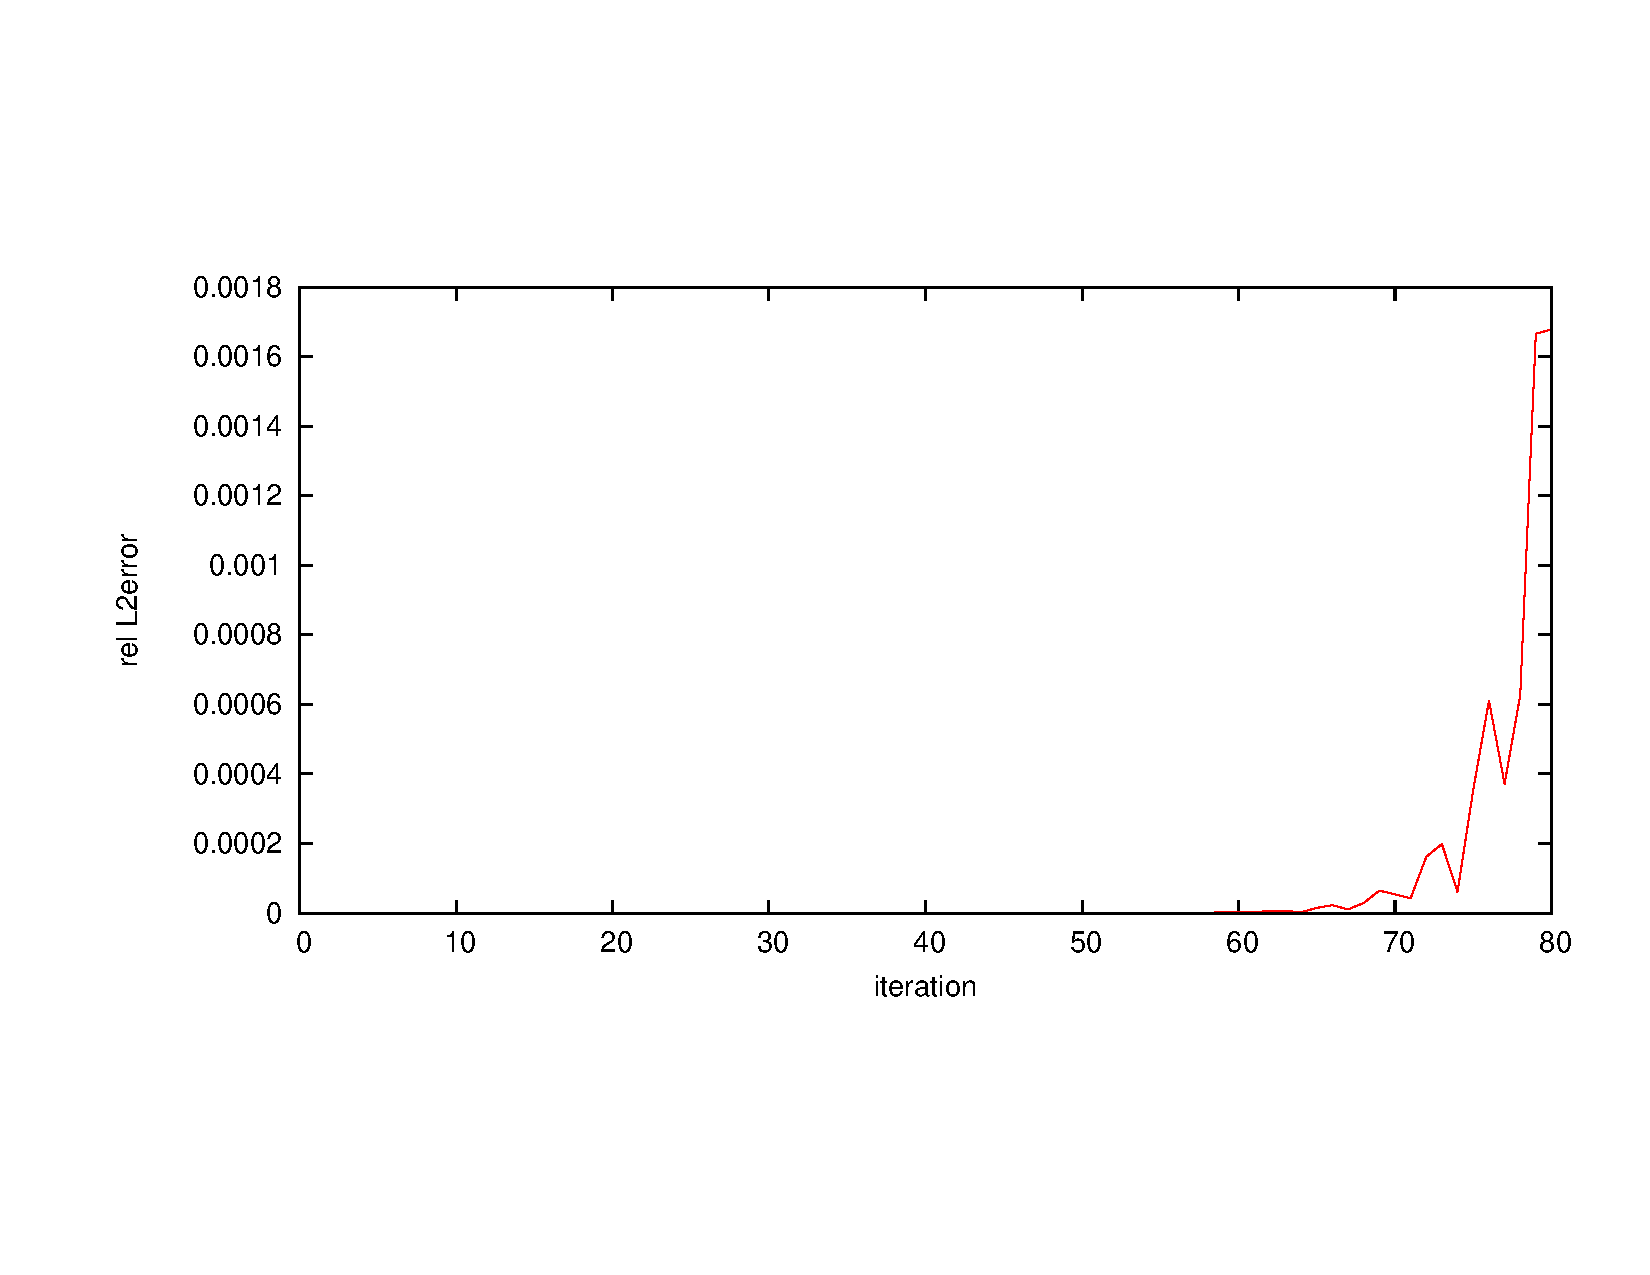
\includegraphics[trim = 2cm 4cm 1cm 4cm, width=1\textwidth]{plots/consisctency_first_try.pdf}
	\caption{Relative $L2$ error on a grid with $h=\frac 1 2$}
	\label{fig: consisctency_first_try}
\end{figure}
Looking at steps shortly before the method diverges one is able see in the solution the underlying grid structure. Everywhere a triangle edge lies sharps edges arise. Besides continuity the solution on two triangles seems independent although the exact solution is absolutely  regular.

As the decoupling approach works for quasilinear methods, so it is a good starting to analyse the main differences. This leads us to the question: How good serves the second derivative of the Poisson solution for an approximation of the second derivative of the exact solution?
We illustrate the significance of this question by a example
\begin{example}
	Let $\tilde u$ be an approximation of $u\in C^2(\R)$ with $u-\tilde u \in \bigO(h)$. 
	%Differentiating twice we are left with $\dxx{x} u(x)-\dxx{x} \tilde u(x)\in \bigO(h^{-1})$ meaning a decrease of the grid size comes along with a increase of the error in the second derivatives.
	%????????//
	Differentiating twice we are left with the taylor approximation
	\begin{align*}
		\dxx{x} u(x)-\dxx{x} \tilde u(x) \approx \frac{\tilde u(x+2h) - 2\tilde u(x) - \tilde u(x-2h) - (u(x+2h) - 2u(x) - u(x-2h))} {4h^2} \\
		 \in \bigO(h^{-1})
	\end{align*}
	This shows, even for small $h$ a good approximation of $u$ does not imply that its second derivatives are good approximations for second derivatives of $u$.
\end{example}

Let us recall the geometric interpretation of the second derivative, it indicates the curvature of a function and hence also describes the convexity, concavity respectively.

One improvement could be the smoothing process during a convexification for it will smooth away all unintended concave curvatures. But probably the result will be still unsatisfiable because convexification does not affect sharp edges at triangle transitions.

Another idea is force more regularity on the first derivative and thus, implicitly obtain a more steady solution. This suits to the ansatz pursued by Neilan described in section \ref{subsec: disrete Hessian}, his proposed correction terms vanish as the gradient jump across internal edges tends to zero.
Hence, we add the following normal derivatives penalty term 
\begin{align}
	\sum_{e \in \edgesi} \sigma_g |e |\int_e \jump{ \nabla u} \jump {\nabla v} \label{eq: grad penalty term}
\end{align}
to the formulation in \eqref{eq: sipg iteration}.
Note, that this avoids variational crimes by interior jumps of derivatives along interior edges of the triangulation. But we implicitly imply that the desired solution is contained in $H^2(\Omega)$, it is not yet clear how this term behaves for less regular solution.
But, indeed with the new penalisation of the gradient the implementation is consistent with the previous example. The consistency check was carried out with the choice $\sigma_g$ equal to $\sigma=30$, as well as for much smaller choices.
%\todo{Noelle gluecklich machen querschnitt}

Nevertheless, starting over with the initial guess from \eqref{eq: start sqrt_f} the method is instable and diverges. But the results yet are very remarkable. As shown in figure \ref{fig: oscillation} the error is oscillating while diverging  to infinity.
\begin{figure}[h]
	\centering
	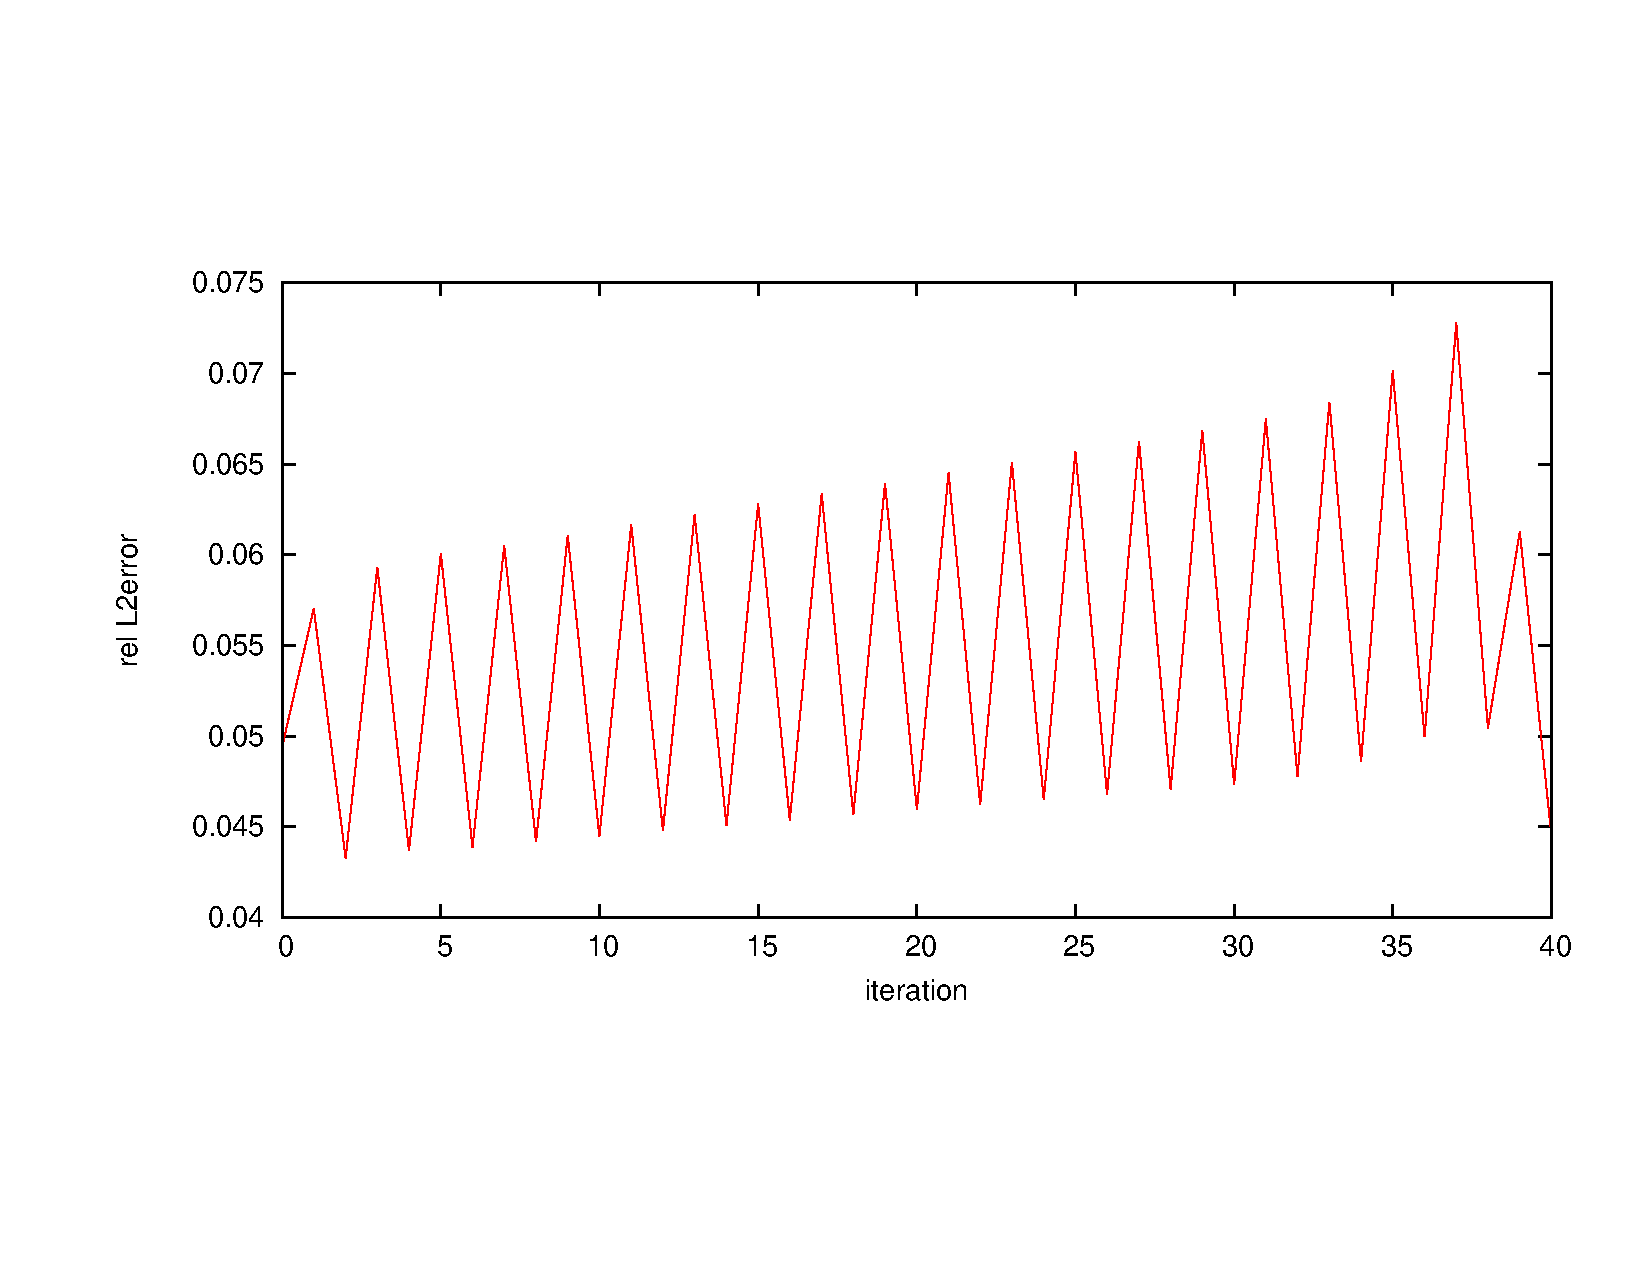
\includegraphics[trim = 2cm 4cm 1cm 4cm, width=1\textwidth]{plots/oscillation.pdf}
	\caption{Relative $L2$ error on a grid with $h=\frac 1 4$ and gradient penalty}
	\label{fig: oscillation}
\end{figure}

\begin{figure}[!h]
\begin{subfigure}[b]{.5\textwidth}
	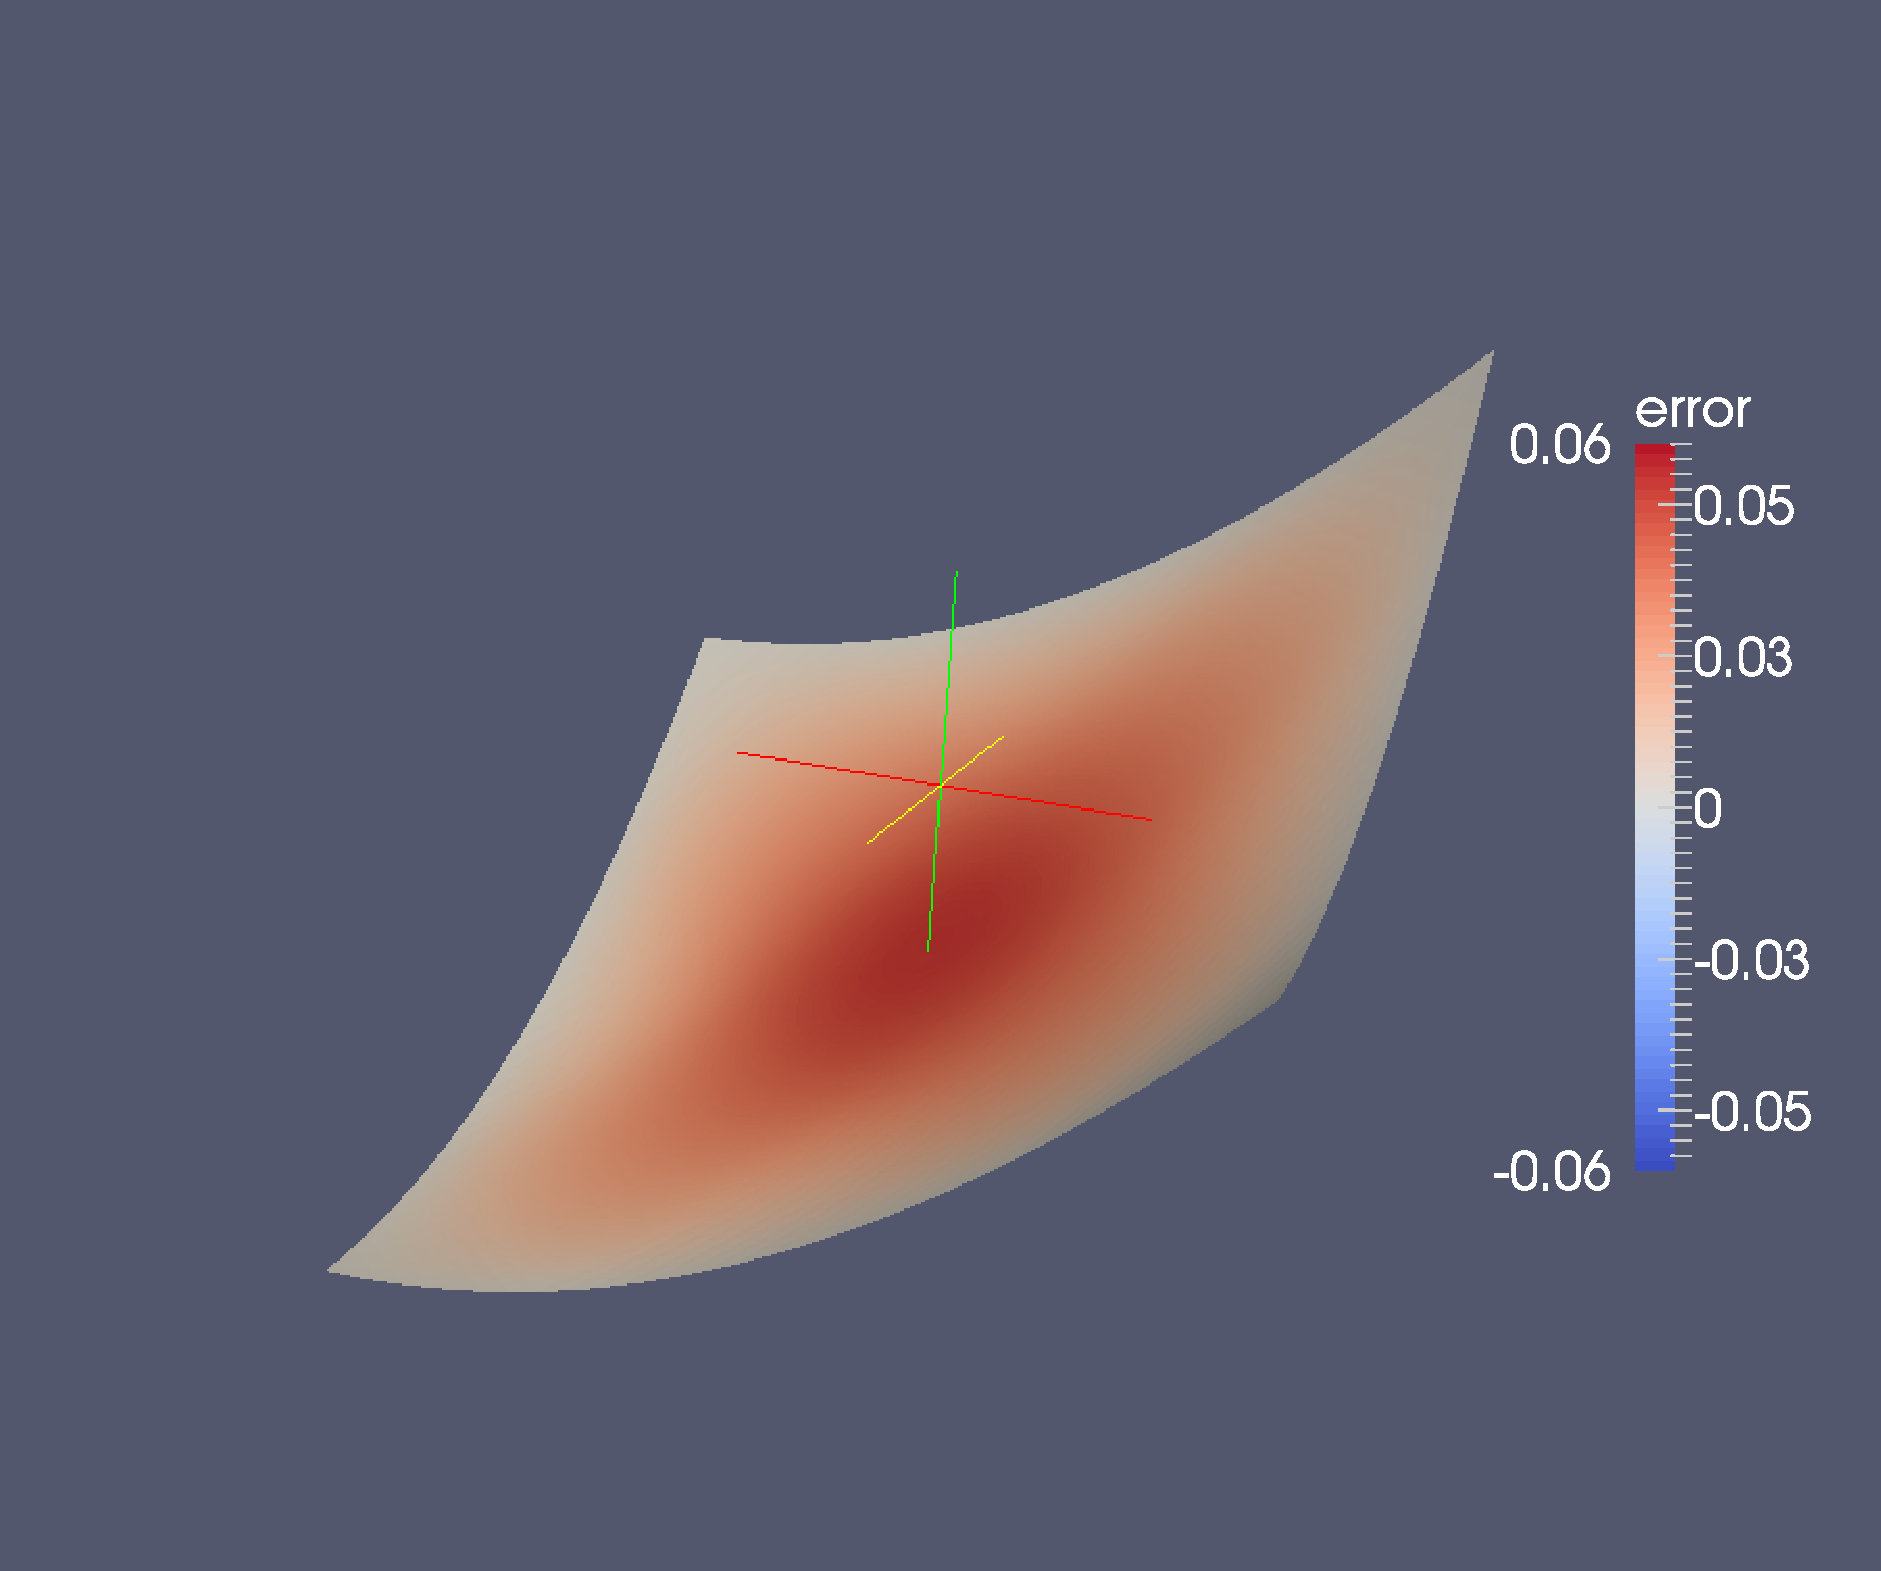
\includegraphics[width=1.\textwidth]{plots/with_penalty_it22.pdf}
	\caption{Solution after 23 steps}
\end{subfigure}
\begin{subfigure}[b]{.5\textwidth}
	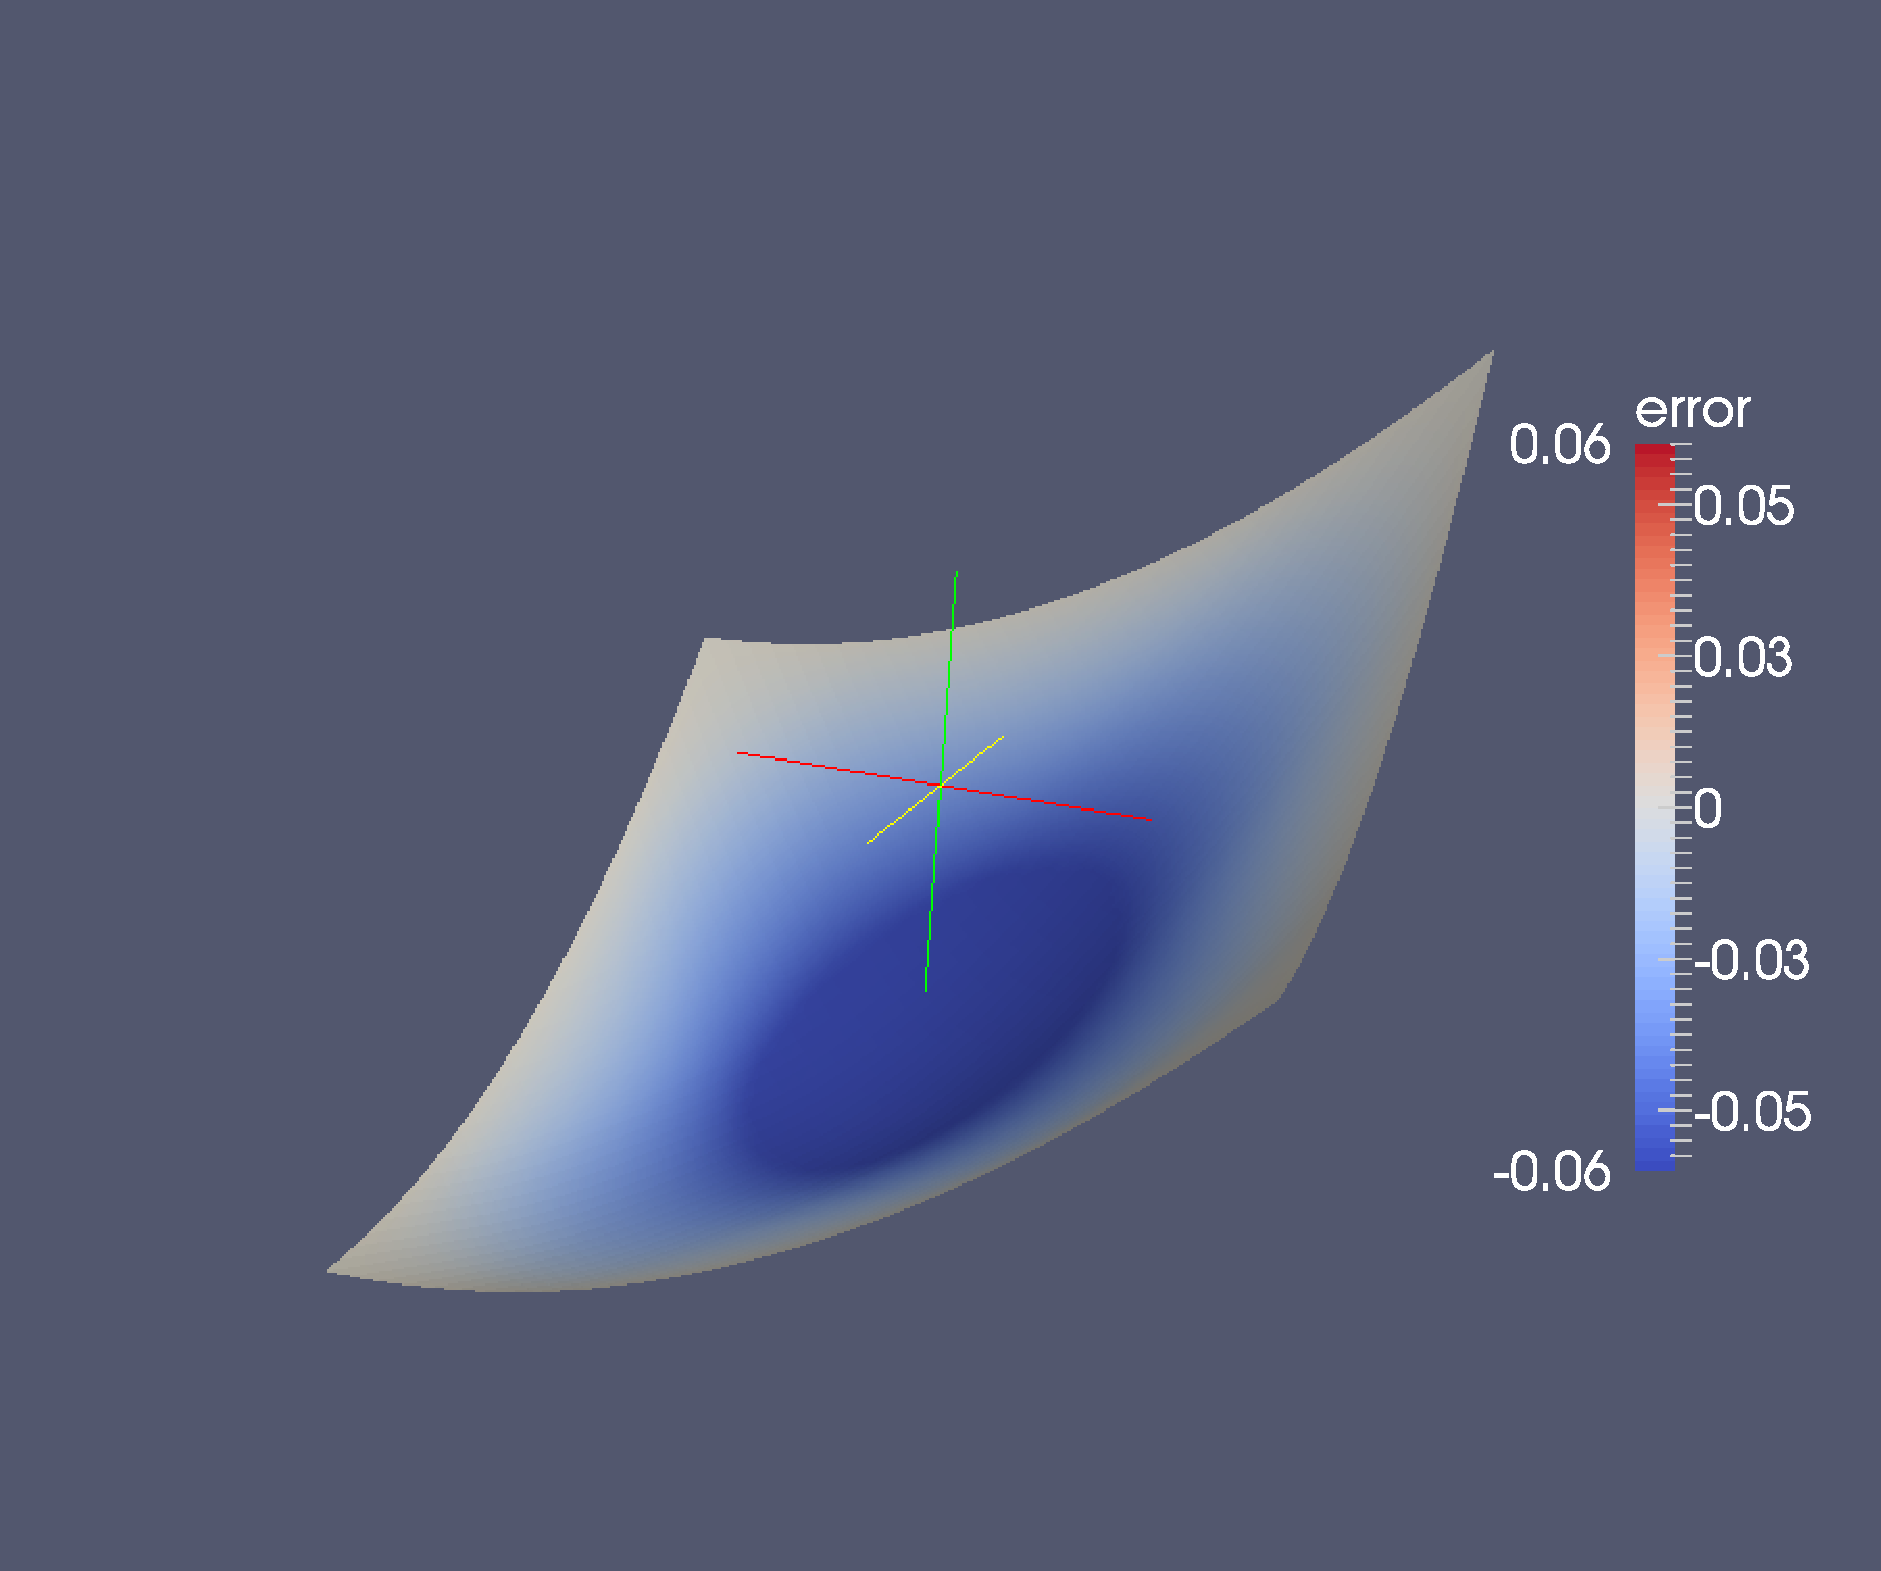
\includegraphics[width=1.\textwidth]{plots/with_penalty_it23.pdf}
	\caption{Solution after 24 steps}
\end{subfigure}
\caption{The solution in two consecutive iterations}
\label{fig: diff iteration}
\end{figure}
Figure \ref{fig: diff iteration} shows to consecutive steps, the error $u-u_{exact}$ is denoted by the surface color. We see that the solution after 23 steps lies above of the exact solution, while one iteration later the Poisson solution lies below of it. These frames are exemplary for the behaviour of our numerical solution. After a step above the solution one below follows, it looks like the solution is split into two subsequences.  And as we have also seen in the devolution of the error, these subsequences seem even to drive each other away from the actual solution.

To prevent our algorithm from doing so we couple the two subsequences by a damping. Before we continue iterating we combine the current solution with the function calculated one step before by an affine composition. Hence we got a further parameter $\alpha$, namely the amount with that the new solution contributes to the iteration.

\subsection{Modification of the Cofactor Matrix}\label{sec: mod cofactor}
For the condition of the problem it is necessary that the eigenvalues of the diffusion matrix, namely $\mycof{D_h^2 u_h^i}$ are positive for all $x$. Even better is if they are constrained from below with some constant $\varepsilon$. 
To suffice this criteria we introduce a modified cofactor matrix
\[ 
	\mycofMod {D^2_h u_h} = \begin{cases}
	\mycof {D^2_h u_h} & \lambda \geq \varepsilon	\\
	\mycof {D^2_h u_h}+ (-\lambda+\varepsilon) Id%\begin{pmatrix} -\lambda+\varepsilon & 0 \\ 0 & -\lambda+\varepsilon \end{pmatrix} 
	& else
	\end{cases}
\]
where $\lambda$ is the minimal eigenvalue of $ \mycof {D^2_h u_h}$ and $Id$ is the $d \times d$-Identity matrix. Now we replace all occurrences of $\mycof {D^2_h u_h}$ in \eqref{eq: sipg iteration} by $\mycofMod {D^2_h u_h}$ to stabilise the problem condition.

\section{The Algorithm}

Bringing those points together our method to carry out the fixed point iteration works as Algorithm \ref{alg: final} describes.

\begin{algorithm}
\begin{algorithmic}
\Require triangulation \triang, desired mesh width $h$, maximimal number of intermediate steps $i_{max}$
\State $u_0\gets $ solution of  $
	\triangle u = \sqrt{2f} \text{ in } \Omega $ with $
	u = g \text{ on }\partial \Omega$
\While {$h < H$}
	\State $i \gets 0$
%	\While {$|u_i-u_{i-1}| < \varepsilon$}
	\While {$i < i_{max} $}
		\State $u_i \gets$ solution of \ref{sec: SIPG} with modified cofactor matrix (\ref{sec: mod cofactor})
		\State $u_i \gets \alpha u_{i-1} + (1-\alpha)u_i $
		\State (convexify)
		\State $i \gets i+1$
	\EndWhile
	\State $h, \triang \gets h/2, \triangFine$
\EndWhile
\end{algorithmic}
\caption{Final Algorithm}
\label{alg: final}
\end{algorithm}

The step convexify is put into brackets for it is not clear whether a convexification is necessary and actually helps the convergence. A lot of the methods mentioned in the chapters \ref{ch:MongeAmpereEq} and \ref{ch:DGMongeAmpere} work without an explicit convexification, although most require a convex initial guess. 
Additionally the approach described in section \ref{subsec: convexification} is intricately to implement, increases significantly the computation costs and it may modify functions even though they already are convex. We note, that for the condition of the stiffness matrix of the used SIPG method we need the cofactor matrix to be positive definit which is equivalent to the piecewise convexity of the last iteration step. However, our modification of the cofactor matrix  may avert the problems arising for slightly non convex intermediate solutions.
